\subsection{Configuration initiale (interface web)}
La suite de la configuration est réalisée au travers de l'interface web :
\begin{itemize}
    \item Se connecter à l'aide des identifiants par défaut (admin|pfsense)
    \item Lancer l'assistant de configuration initiale
    \item Choisir le nom d'hôte, le nom de domaine et les serveurs DNS (figure \ref{fig:03-config-web-01})
    \item Choisir un serveur NTP et un fuseau horaire ("Etc/UTC")
    \item Définir la configuration de l'interface WAN
    \item Définir la configuration de l'interface LAN
    \item Définir le mot de passe d'administration
    \item Recharger PFSense
    \item Accéder à "System/Package Manager"
    \item Accéder à "Available Package"
    \begin{itemize}
        \item Installer les additions invitées (uniquement pour un hyperviseur VMware) : "Open-VM-Tools"
        \item Installer la gestion du clavier "Shellcmd"
        \item Accéder à la configuration du service "Shellcmd" et ajouter la commande suivante (figure 13)
    \end{itemize}
\end{itemize}

\begin{lstlisting}[language=bash,caption={Définition du clavier français}]
kbdcontrol -l /usr/share/syscons/keymaps/fr.iso.kbd
\end{lstlisting}

\begin{figure}[H]
    \centering
    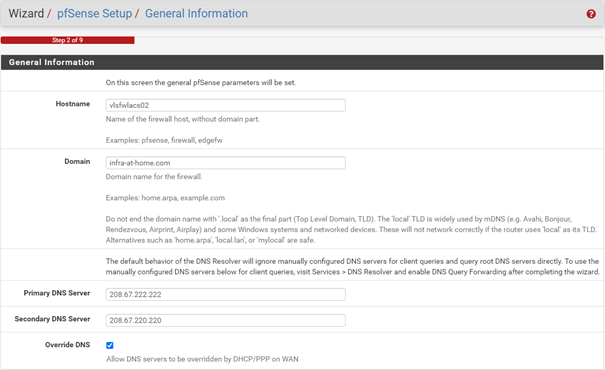
\includegraphics[width=1.0\textwidth]{03-Installation/Images/03-config-web-01.png}
    \caption{Configuration web - Nom d'hôte, de domaine et serveurs DNS}
    \label{fig:03-config-web-01}
\end{figure}

\begin{figure}[H]
    \centering
    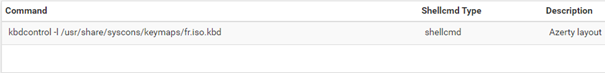
\includegraphics[width=1.0\textwidth]{03-Installation/Images/03-config-web-02.png}
    \caption{Configuration web - Configuration du clavier en disposition AZERTY}
    \label{fig:03-config-web-02}
\end{figure}

\begin{tip}
    Si la configuration est réalisée sur un réseau privé, il est important de permettre le trafic en provenance de réseaux privés sur l'interface WAN.
\end{tip}
